\subsection{Solve a real problem}
Once the relevance has been demonstrated, we consider the benefits and advantages that the use of the data as a user can bring us.
This objective requires meticulous work both to discover it and to transmit these concepts to the user in a clear way,
simple and direct and thus achieve a link that increases the curiosity of the user to deepen the subject and
stay informed.

It is very important to stay in the user's place and discover what is really necessary for him. Only if the user understands the relevance of
the data and the influence that these have in their daily life, a commitment on the part of this will be possible.

That is, the information should cover a need of the user, even if the user does not know a priori that he has this need. Maybe it's
Our goal is to let he see how useful and advantageous this data usage can be.

When we have some data that is updated periodically, we must think in what way the fluctuation may interest us or that certain
changes Here comes the representation of the information in a way that awakens the need for data monitoring by
of the user.

\subsubsection*{Suggested strategies} 
First of all discover in what way the data can help users. Next we have to find a way to let him see
because they are important to him and how he can benefit from using them in his daily life.
If the data is updated periodically, it is necessary to analyze what type of variations are important in the user's daily life.
Conduct a market study and see if there are already products that offer this information. If this is the case, it will be analyzed because
It is attractive to the user and try to improve it.

\subsubsection*{In the context of Aire Guru \ldots} 
The user is offered a platform that indicates his exposure to totally customized air pollution if the need to carry
no device for reading pollutans.



Air Guru with explicit permission to read the location by the user, pick up the polygon where
the user is found and stores the most recent pollution measure for that polygon. Next, the
user can view the exposure to the pollution to which he has been subjected.
\begin{figure}[ht]
    \centering 
    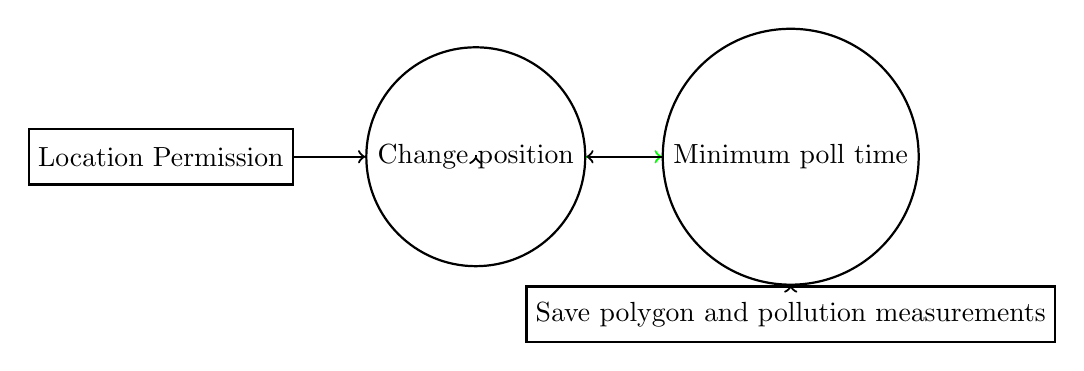
\begin{tikzpicture}[thick]
        \node[draw,rectangle,minimum size=20] (a) {Location Permission};
         \node[draw,circle,minimum size=6,right of= a, node distance=4cm] (b) {Change position};
         \node[draw,circle,minimum size=5,right of= b, node distance=4cm] (c) {Minimum poll time};
         \node[draw,rectangle,minimum size=20,below of=c, node distance=2cm] (d) {Save polygon and pollution measurements};
         \draw[->] (a) to (b);
         \draw[->] (b) to (b);
        \draw[->,green] (b) to (c);
        \draw[->] (c) to (d);
     \draw[->] (c) to (b);
      \end{tikzpicture}
      \caption{Collecting user location}
    \end{figure}
    \begin{figure}[ht]
        \centering
        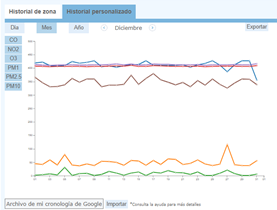
\includegraphics[width=8cm]{importedDataDecember}
        \caption{Personal Records. December}
    \end{figure}
    We can see the exposure to air pollution since 2018 without having to have been using the tool since
    Using the import Google chronology button, we can import the location history provided by the
    pollution that has been exposed since 2018. In the help section we can find a guide how to
    export and import this history of locations.
\elsparagraph{Evaluation}  
\begin{itemize}
    \done Unique feature, fully customized pollution exposure monitoring
    \done Description of the effects, polluting sources, description of the pollutans in a single platform
    \crossed Presenting how exposure to pollution can be reduced more specifically
    
\end{itemize}